\documentclass[11pt,a4paper]{article}
\usepackage[utf8]{inputenc}
\usepackage[spanish]{babel}
\usepackage{amsmath}
\usepackage{amsfonts}
\usepackage{float}
\usepackage{amssymb}
\usepackage{graphicx}
\usepackage[left=2cm,right=2cm,top=2cm,bottom=2cm]{geometry}
\author{Marina Esgueva Ruiz}
\title{Centros con parámetro de forma variable}
\begin{document}
\begin{table}
\caption{$\epsilon$ fijo en todo el dominio.}
\centering
\begin{tabular}{|c|c|c|c|}
\hline
\ $N$ & ECM & Condicionamiento & $\epsilon$ \\
\hline
\ 15 &  3.7947e-03& 1.1330e+07& 4.6964e-01\\
\ 16 & 4.3621e-03 & 1.4510e+07 & 4.6985e-01 \\
\ 17 & 2.0315e-03 & 9.9491e+07 & 4.0195e-01 \\
\ 18 &  2.0728e-03 & 7.4882e+07 &  4.3862e-01 \\
\ 19 & 2.1151e-03 & 1.8219e+07& 5.2016e-01 \\
\ 20 & 2.3713e-03 &  2.7216e+07&5.0122e-01 \\
\ 21 & 1.5430e-03 & 5.6210e+07 & 4.9027e-01 \\
\ 22 & 1.5929e-03 & 9.0357e+07 &  5.1272e-01 \\
\ 23 &  1.3684e-03 & 1.3074e+08 & 4.9681e-01 \\
\ 24 &  7.3919e-04 & 2.7533e+10 & 3.1520e-01 \\
\ 25 & 2.9188e-04 & 9.6904e+09 & 3.4840e-01 \\
\ 30 & 1.1801e-04 & 1.4361e+12 &  3.0784e-01 \\
\ 35 & 4.1852e-05 & 1.6529e+12 & 3.4519e-01 \\ 
\hline

\end{tabular}
\end{table}

\begin{figure}[H]
\centering

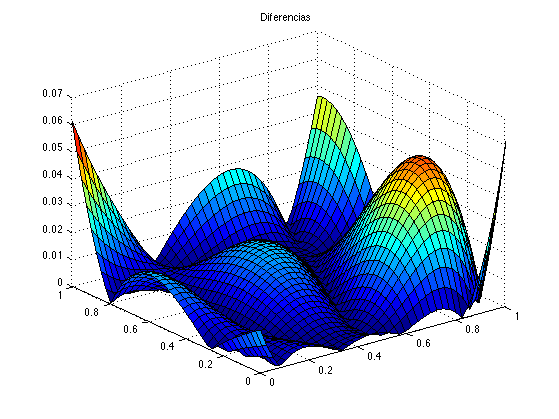
\includegraphics[scale=0.35]{diferencias15.png}
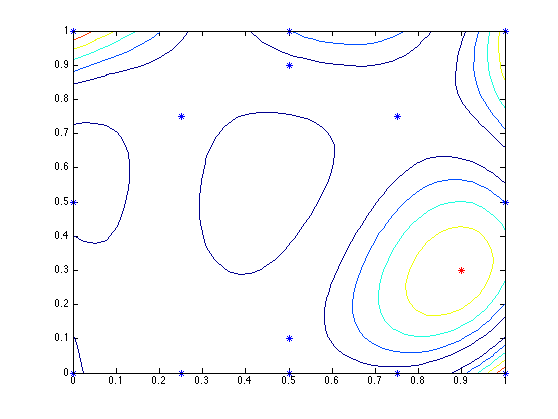
\includegraphics[scale=0.35]{centros15.png}
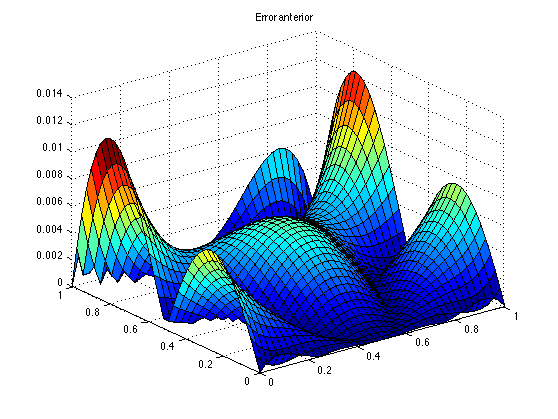
\includegraphics[scale=0.35]{error15.png}
\caption{15 centros}
\end{figure}
\begin{figure}[H]
\centering

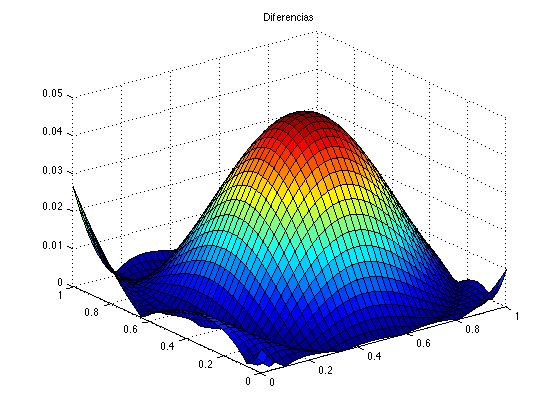
\includegraphics[scale=0.35]{diferencias16.png}
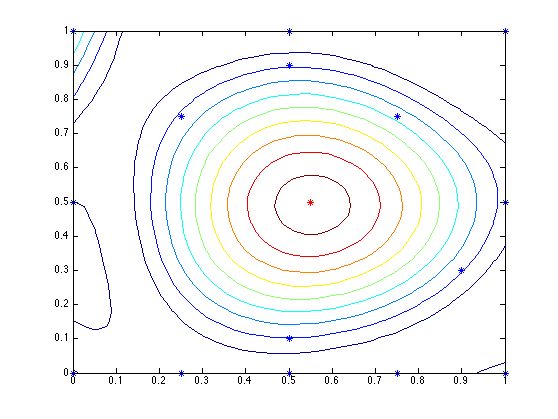
\includegraphics[scale=0.4]{centros16.png}
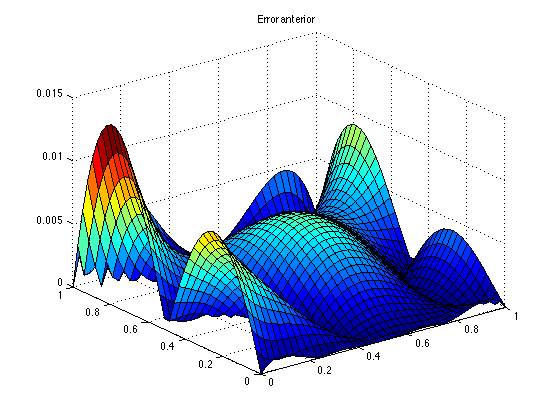
\includegraphics[scale=0.4]{error16.png}
\caption{16 centros}
\end{figure}

\begin{figure}[H]
\centering

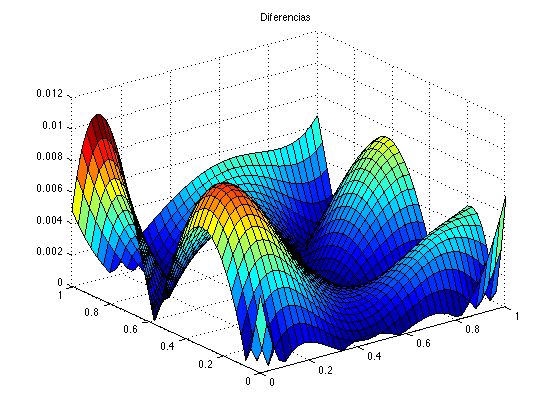
\includegraphics[scale=0.35]{diferencias17.png}
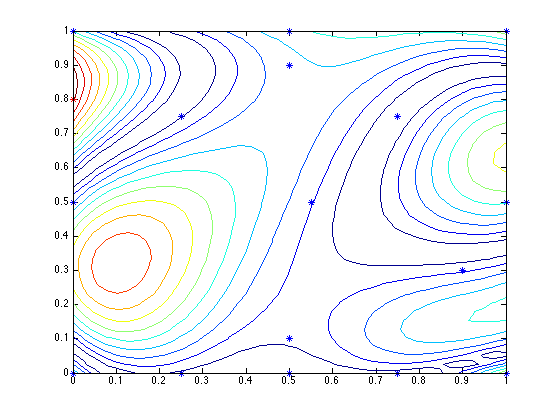
\includegraphics[scale=0.35]{centros17.png}
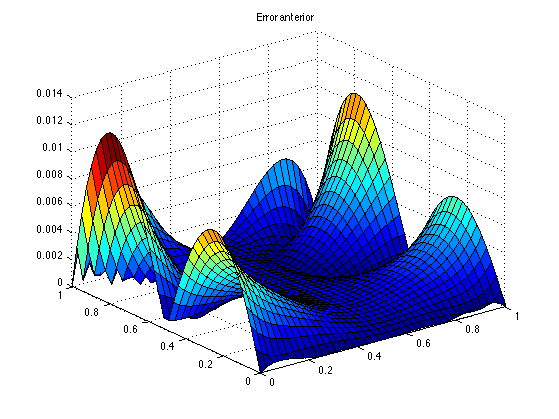
\includegraphics[scale=0.35]{error17.png}
\caption{17 centros}
\end{figure}

\begin{figure}[H]
\centering

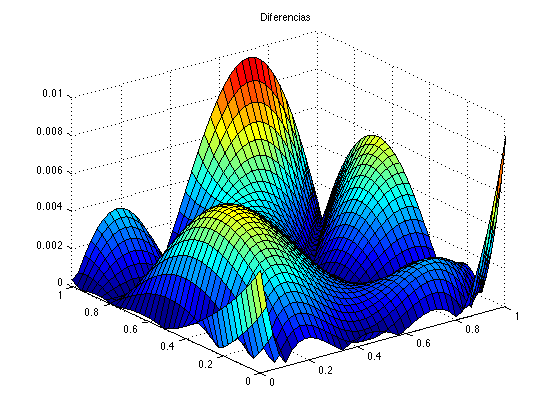
\includegraphics[scale=0.35]{diferencias18.png}
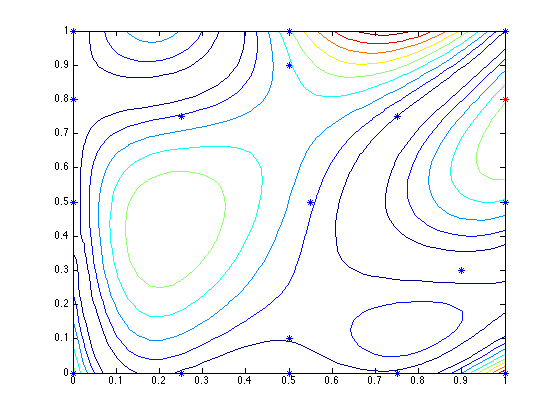
\includegraphics[scale=0.35]{centros18.png}
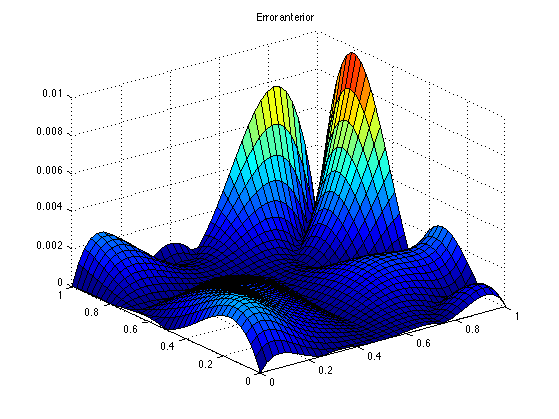
\includegraphics[scale=0.35]{error18.png}
\caption{18 centros}
\end{figure}

\begin{figure}[H]
\centering

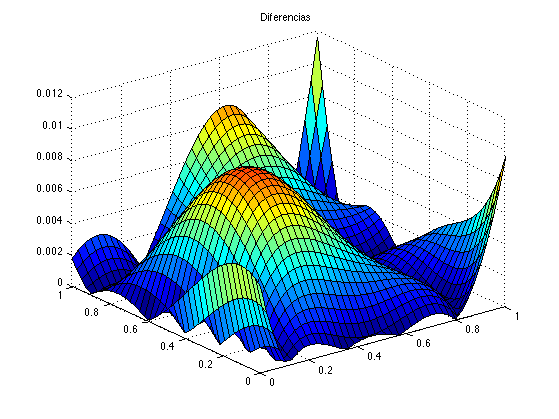
\includegraphics[scale=0.35]{diferencias19.png}
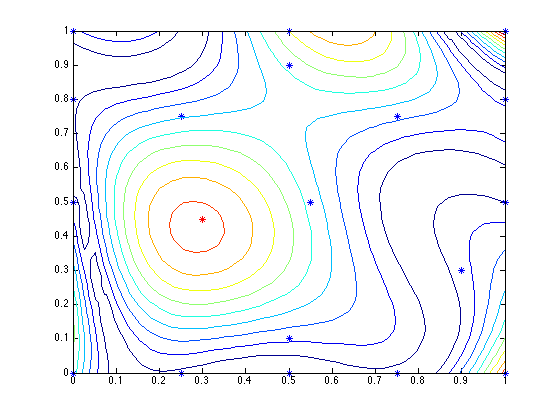
\includegraphics[scale=0.35]{centros19.png}
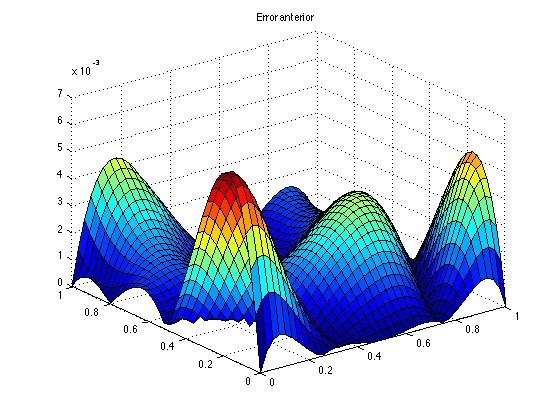
\includegraphics[scale=0.35]{error19.png}
\caption{19 centros}
\end{figure}

\begin{figure}[H]
\centering

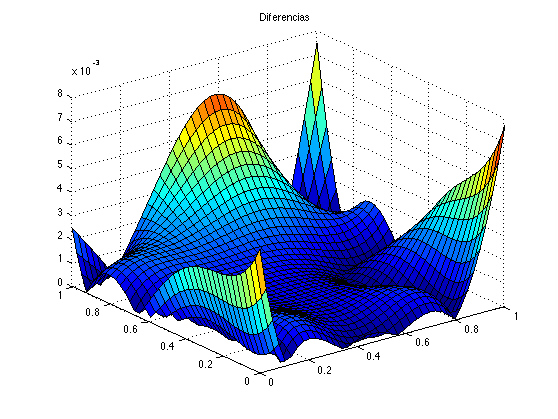
\includegraphics[scale=0.35]{diferencias20.png}
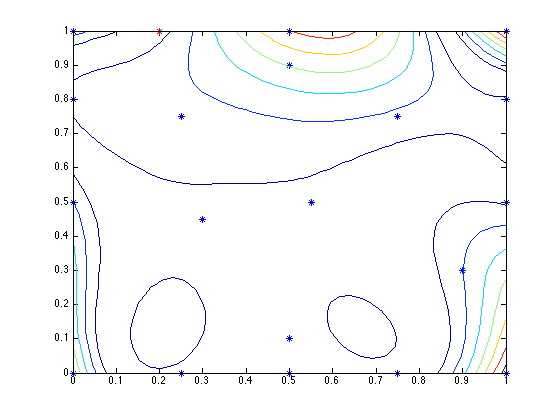
\includegraphics[scale=0.35]{centros20.png}
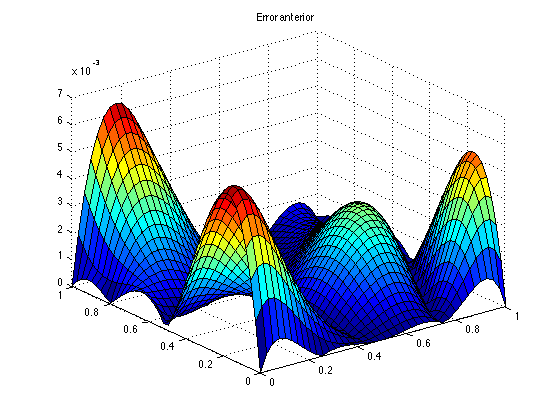
\includegraphics[scale=0.35]{error20.png}
\caption{20 centros}
\end{figure}

\begin{figure}[H]
\centering

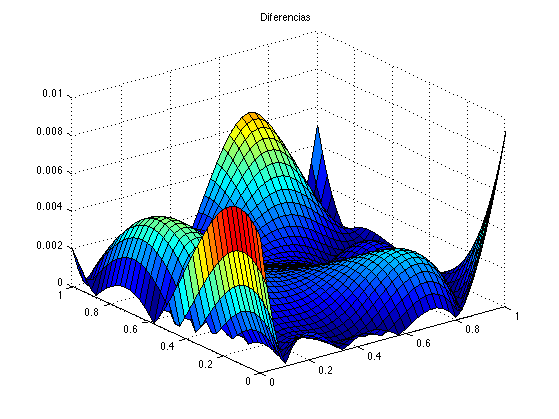
\includegraphics[scale=0.35]{diferencias21.png}
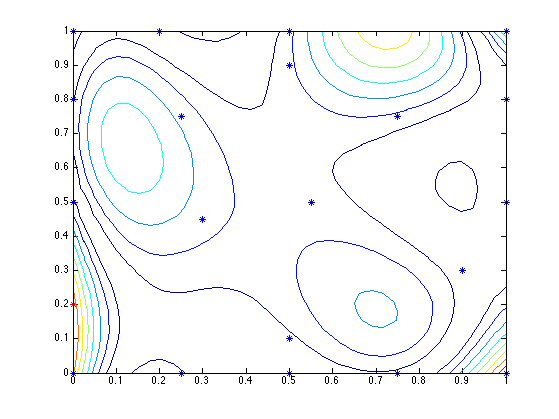
\includegraphics[scale=0.35]{centros21.png}
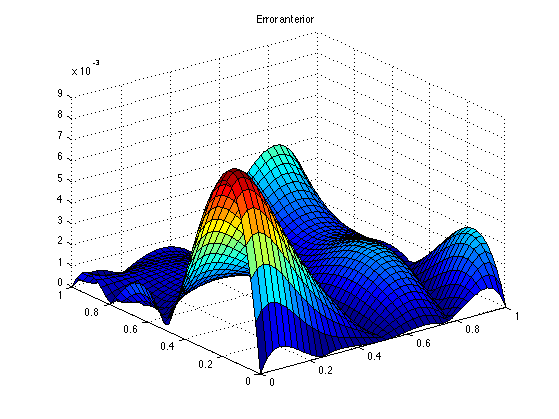
\includegraphics[scale=0.35]{error21.png}
\caption{21 centros}
\end{figure}

\begin{figure}[H]
\centering

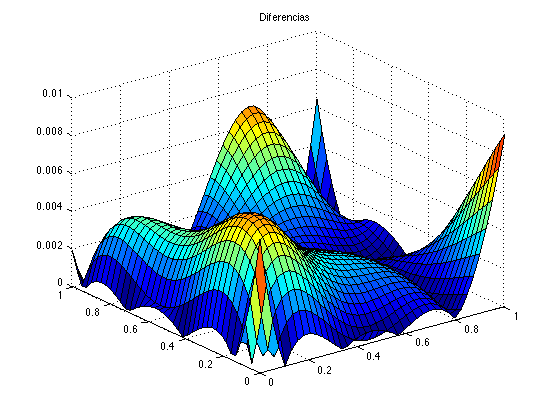
\includegraphics[scale=0.35]{diferencias22.png}
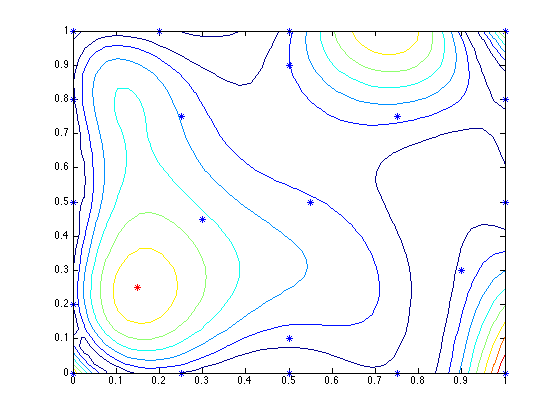
\includegraphics[scale=0.35]{centros22.png}
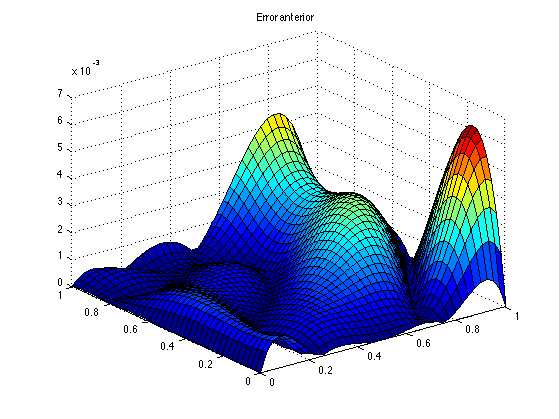
\includegraphics[scale=0.35]{error22.png}
\caption{22 centros}
\end{figure}

\begin{figure}[H]
\centering

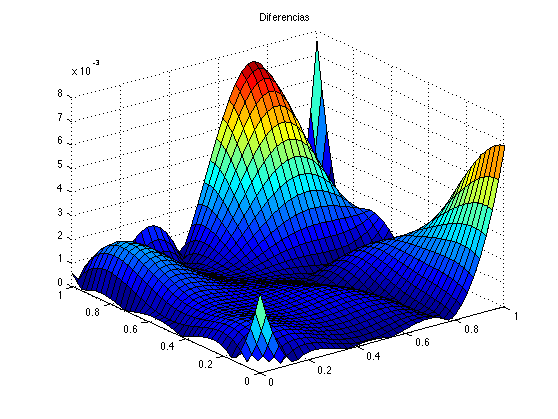
\includegraphics[scale=0.35]{diferencias23.png}
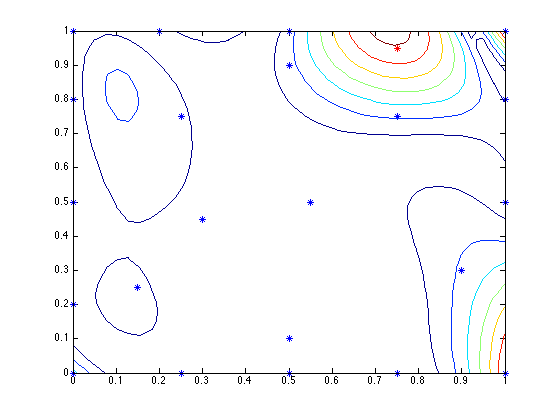
\includegraphics[scale=0.35]{centros23.png}
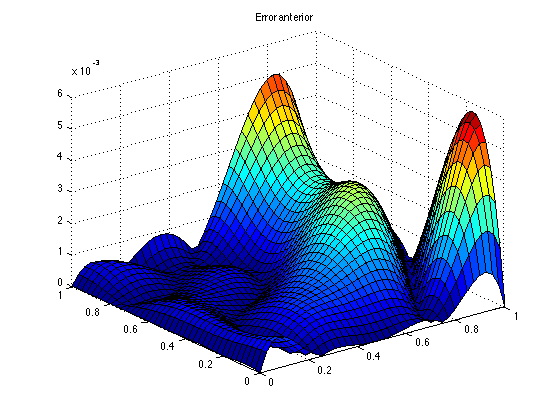
\includegraphics[scale=0.35]{error23.png}
\caption{23 centros}
\end{figure}

\begin{figure}[H]
\centering

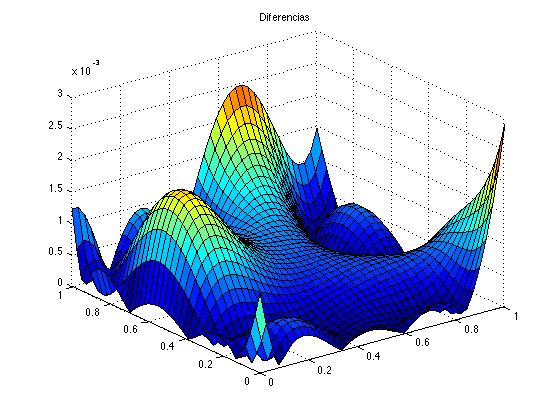
\includegraphics[scale=0.35]{diferencias24.png}
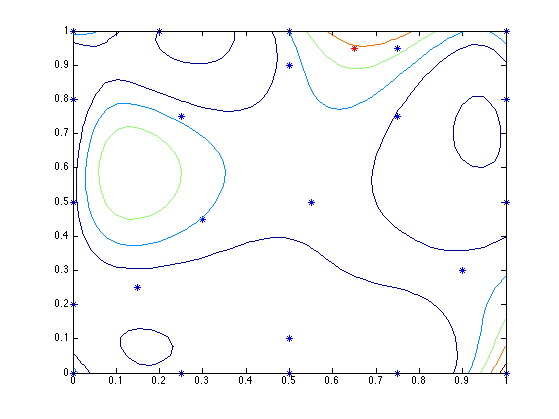
\includegraphics[scale=0.35]{centros24.png}
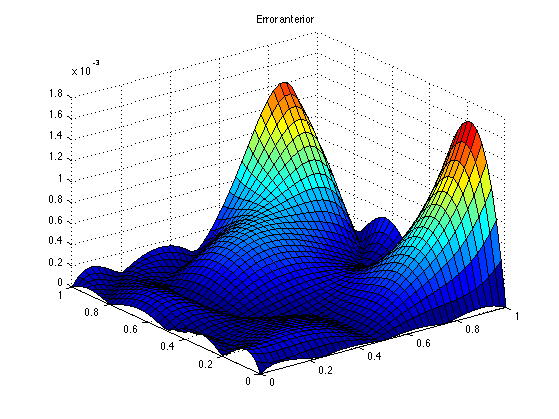
\includegraphics[scale=0.35]{error24.png}
\caption{24 centros}
\end{figure}

\begin{figure}[H]
\centering

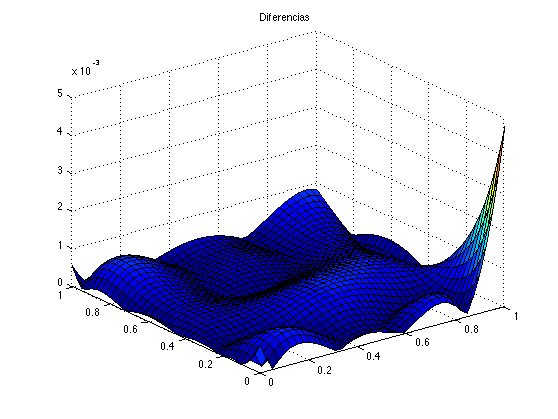
\includegraphics[scale=0.35]{diferencias25.png}
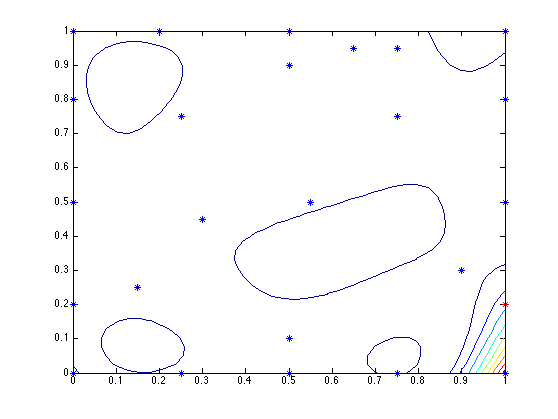
\includegraphics[scale=0.35]{centros25.png}
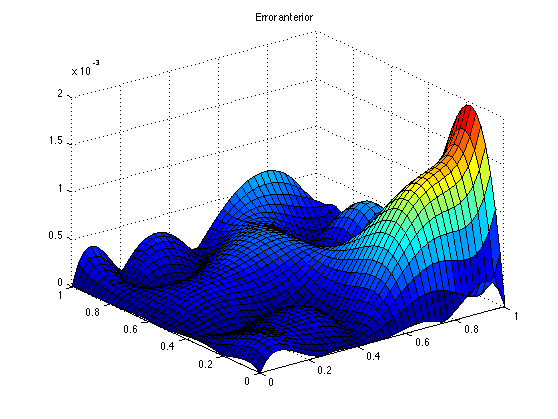
\includegraphics[scale=0.35]{error25.png}
\caption{25 centros}
\end{figure}

\begin{figure}[H]
\centering

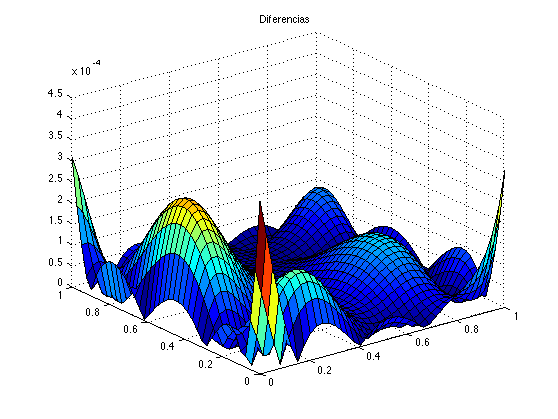
\includegraphics[scale=0.35]{diferencias30.png}
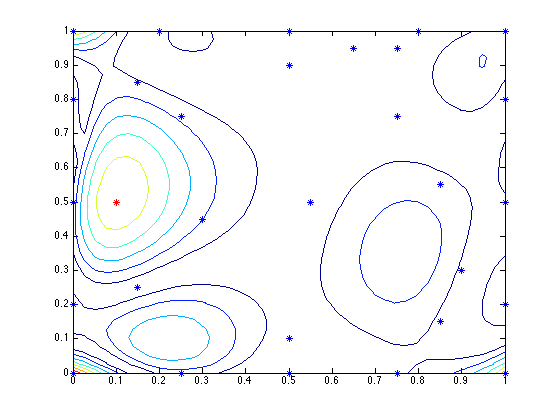
\includegraphics[scale=0.35]{centros30.png}
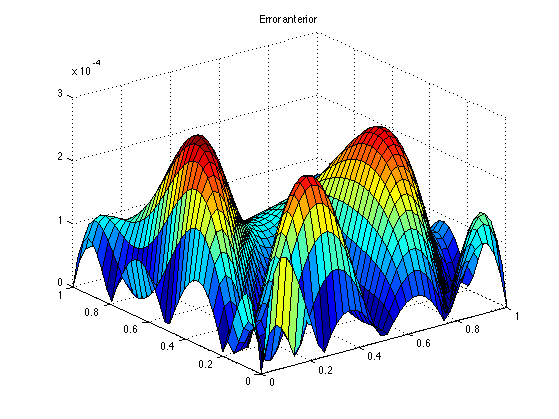
\includegraphics[scale=0.35]{error30.png}
\caption{24 centros}
\end{figure}

\begin{figure}[H]
\centering

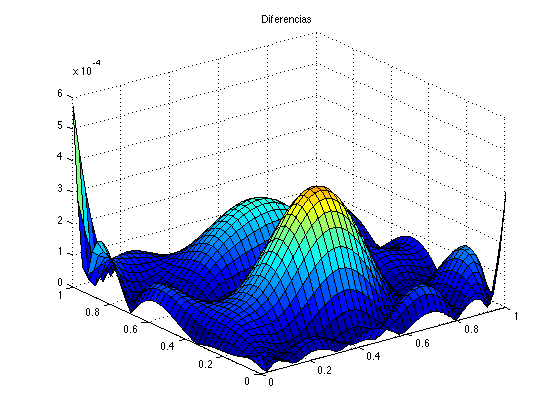
\includegraphics[scale=0.35]{diferencias35.png}
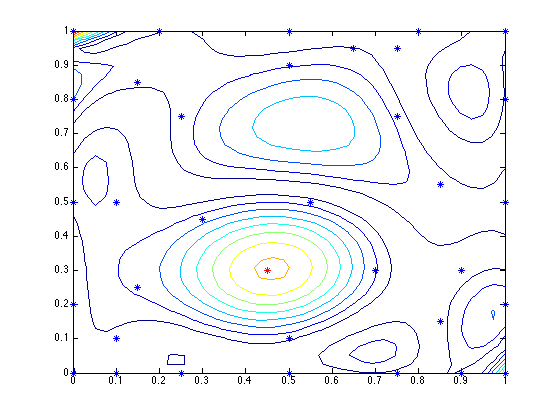
\includegraphics[scale=0.35]{centros35.png}
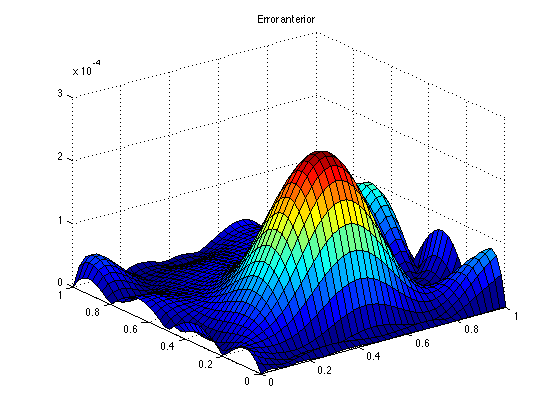
\includegraphics[scale=0.35]{error35.png}
\caption{25 centros}
\end{figure}





\begin{table}
\caption{$\epsilon$ fijo en todo el dominio.}
\centering
\begin{tabular}{|c|c|c|c|}
\hline
\ $N$ & ECM & Condicionamiento & $\epsilon$ \\
\hline
\ 14 &1.0269e-01 & 6.7427e+02 & 1.8314 \\
\ 15 & 1.1231e-01 & 7.9880e+02 & 1.8833 \\
\ 16 & 8.1312e-02 & 9.7180e+02 & 1.8829 \\
\ 17 & 7.1661e-02 & 1.2750e+03 & 1.7701 \\
\ 18 &  9.8397e-02 & 1.4945e+03 & 1.7402 \\


\end{tabular}
\end{table}



\end{document}